\section{Desarrollo / Análisis de Resultados}
\subsection{Análisis de SW}
\begin{figure}[H]
    \centering
    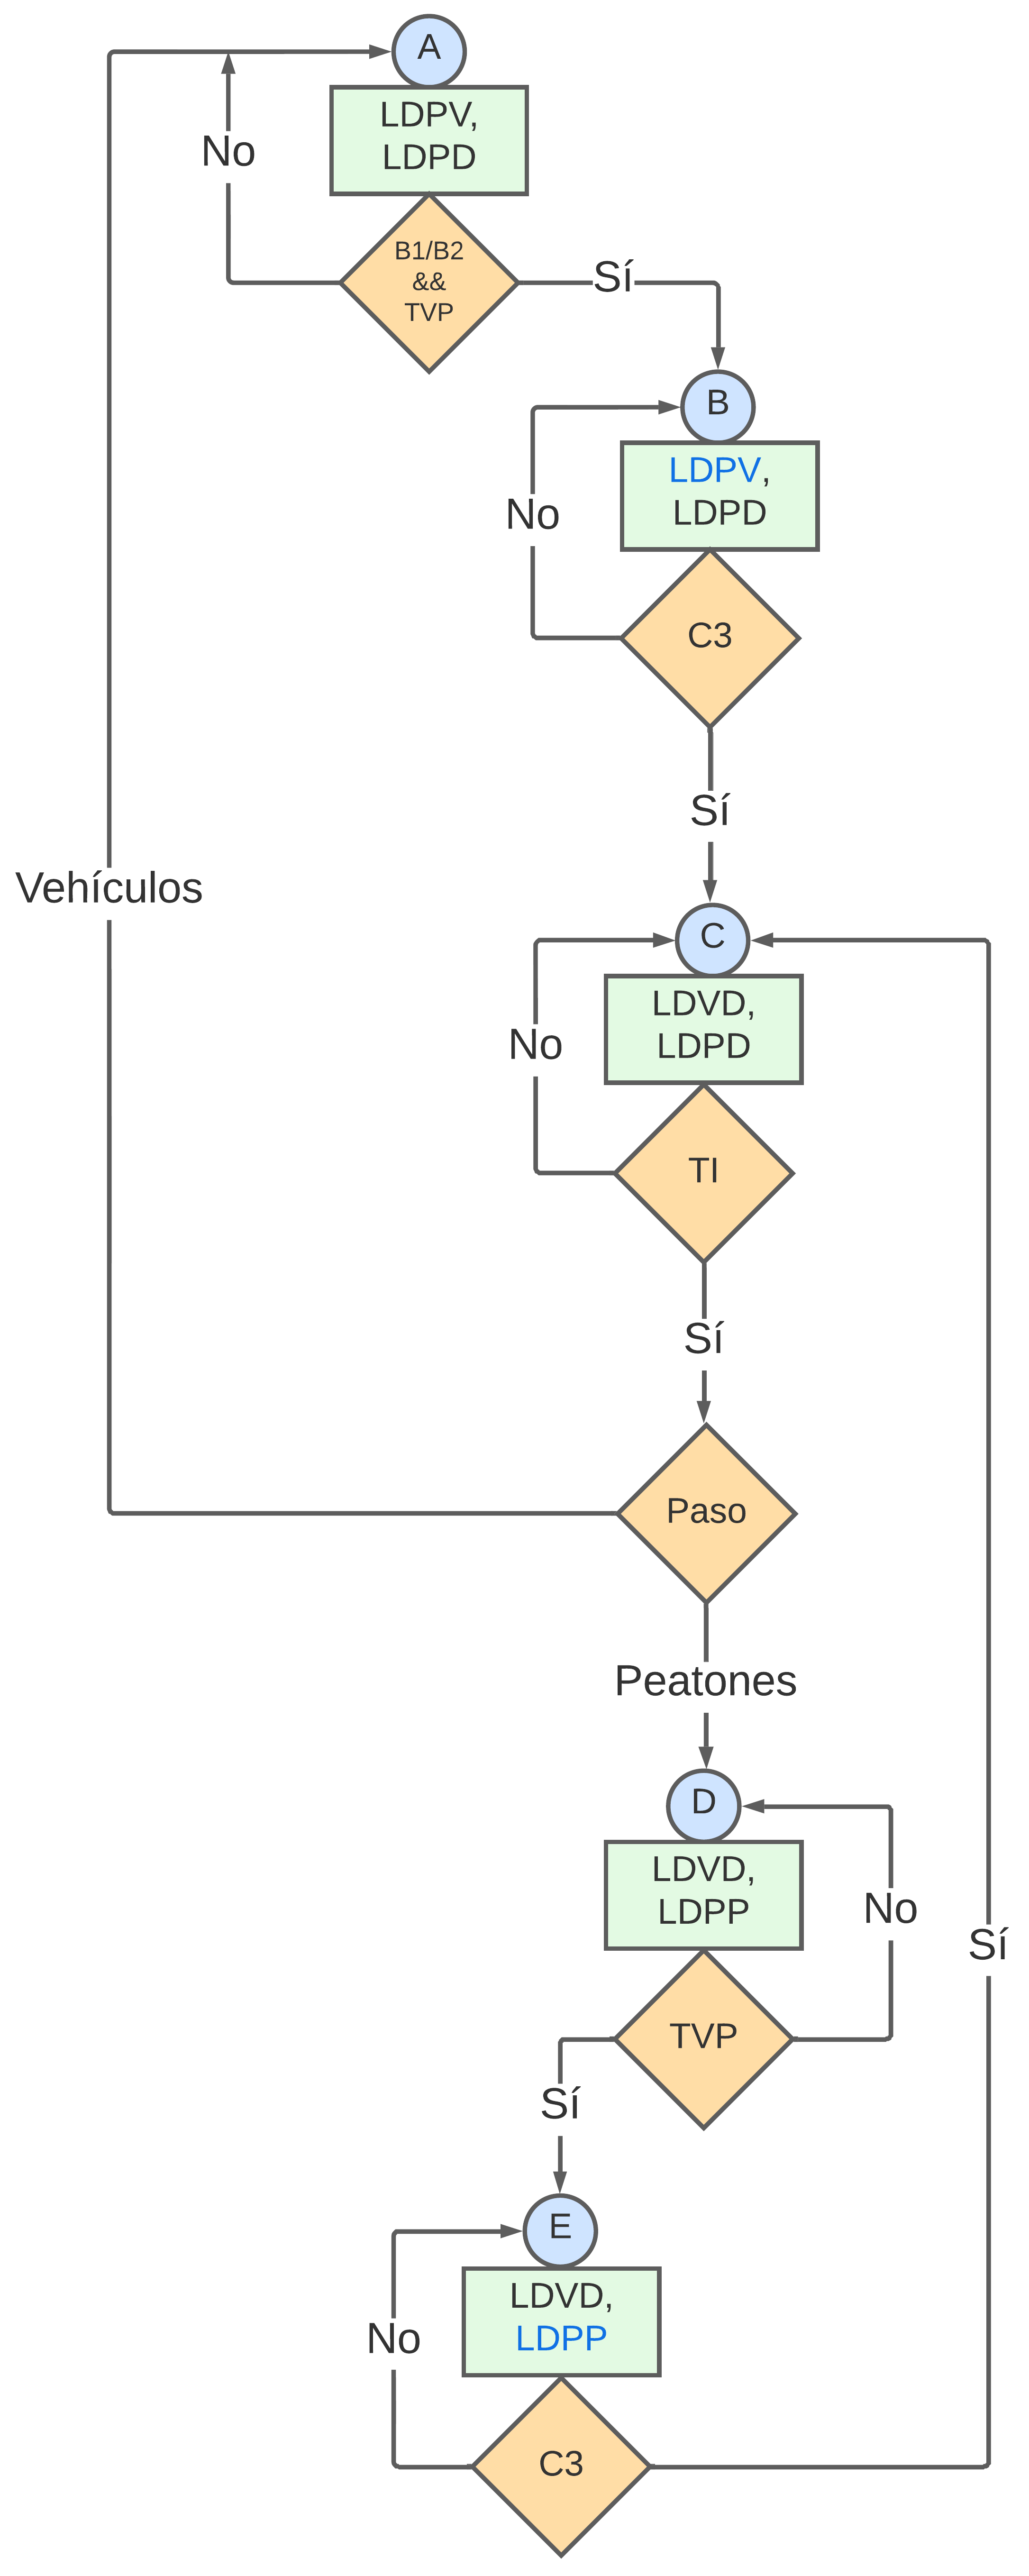
\includegraphics[width=0.7\textwidth]{images/diagrama_asm.png}
    \caption{Diagrama ASM propuesto para el cruce de semáforos. Creación propia}
    \label{diagrama_asm}
\end{figure}

En la figura \ref{diagrama_asm} se puede observar el diagrama ASM construido para el cruce de semáforos mostrado en la figura \ref{cruce_semaforos}. En la siguiente tabla se presenta la descripción de la nomenclatura empleada en el diseño del diagrama: 

\begin{table}[H]
\centering
\renewcommand{\arraystretch}{1.25}
\begin{tabular}{|c|c|c|}
\hline
\multirow{5}{*}{Entradas} & B1   & Botón de semáforo peatonal 1                                                                                             \\ \cline{2-3} 
                          & B2   & Botón de semáforo peatonal 2                                                                                             \\ \cline{2-3} 
                          & TVP  & Timer de paso de vehículos o peatones (10 segundos)                                                                      \\ \cline{2-3} 
                          & TI   & Timer de 1 segundo                                                                                                       \\ \cline{2-3} 
                          & C3   & Contador de parpadeos (cuenta hasta 3)                                                                                   \\ \hline
\multirow{4}{*}{Salidas}  & LDPV & Led de paso de vehículos                                                                                                 \\ \cline{2-3} 
                          & LDPD & Led de peatones detenidos                                                                                                \\ \cline{2-3} 
                          & LDVD & Led de vehículos detenidos                                                                                               \\ \cline{2-3} 
                          & LDPP & Led de paso de peatones                                                                                                  \\ \hline
\multirow{8}{*}{Estados}  & A    & Paso de vehículos por al menos 10 segundos                                                                               \\ \cline{2-3} 
                          & B    & No se han presionado B1 ni B2 y ya pasó el tiempo TV                                                                     \\ \cline{2-3} 
                          & C    & Ya se presionó B1 o B2 y no ha pasado el tiempo TV                                                                       \\ \cline{2-3} 
                          & D    & \begin{tabular}[c]{@{}c@{}}Parpadeo de LDPV para cambio\\ de paso de vehículos a peatones\end{tabular}                   \\ \cline{2-3} 
                          & E    & \begin{tabular}[c]{@{}c@{}}Vehículos y peatones detenidos por \\ 1 segundo para posterior paso de peatones\end{tabular}  \\ \cline{2-3} 
                          & F    & Paso de peatones por al menos 10 segundos                                                                                \\ \cline{2-3} 
                          & G    & \begin{tabular}[c]{@{}c@{}}Parpadeo de LDPP para cambio\\ de paso de peatones a vehículos\end{tabular}                   \\ \cline{2-3} 
                          & H    & \begin{tabular}[c]{@{}c@{}}Vehículos y peatones detenidos por \\ 1 segundo para posterior paso de vehículos\end{tabular} \\ \hline
\end{tabular}
\caption{Entradas, salidas y estados del diagrama ASM propuesto. Creación propia}
\renewcommand{\arraystretch}{1}
\end{table}
\subsection{Análisis de HW}

Analizar el esquemático y sus componentes con osciloscopios y multimetros